\subsubsection{Retrieving the Points of Interests Dataset}

We used the Google Maps API as the data source for our application
because of its accuracy and updated dataset compared with the other
approaches and other APIs ~\cite{googleSite, iltifat2014generation}. In addition, the nearby search
endpoint allows the app to search
for places of a given category within a specified
area. In order to retrieve the places for the
application, eight requests are made, each requesting
places of different categories.
To solve the issues with
time windows, we split the
endpoints into two categories. Five of the requests represent places shown as
part of the itinerary during the day:

\begin{center}
    
\textit{beaches, natural sights, museums, shopping malls and cafeterias.}
\end{center}

and the rest represent places shown
during the night: 

\begin{center}
\textit{nightclubs, bars and restaurants}. 
    
\end{center}

\begin{table}
\caption{Sample Query being made to the google maps nearby search endpoint} \label{t:tab}

\centerline{
  \begin{tabular}{|l|c|c|} 
 \hline
  \textbf{Key} & \textbf{Value} \\ 
 \hline
 location & 35.93575, 14.3754 \\ 
 radius& 50000 \\ 
 type & cafe \\ 
 keyword & must visit tourist \\ 
 \hline
  \end{tabular}
}
\label{SampleQuery}
\end{table}

Table~\ref{SampleQuery} shows the query parameters 
used to gather cafeteria related places in Malta. These
categories are based on the ones used by Wörndl et al.~\cite{Worndl2017} for their
application.




%\begin{figure}[h]
%\centering
%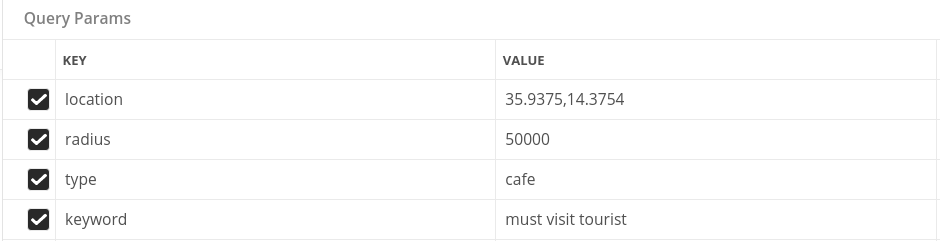
\includegraphics[width=0.8\textwidth]{SampleQuery.png}
%\caption{Sample Query being made to the google maps nearby search endpoint}
%\label{SampleQuery}
%\end{figure}


In return, the API returns a list of places of the specified area and category
and attributes about each place. The attributes used by our application include
the place's name, rating, the number of reviews and the coordinates. 
%\begin{lstlisting}

  %"results": [
    %{
      %"location": {
          %"lat": 35.9204876,
          %"lng": 14.3433952
        %},
      %"name": "Gnejna Bay Beach",
      %"rating": 4.4,
      %"types": ["natural_feature", "point_of_interest"]
      %"user_ratings_total": 1542,
    %}, 
    %...
    %]


%\end{lstlisting}

%%%TODO: Add figure
%Figure X shows an example of a response from the API.\

